\documentclass[tikz,border=16pt]{standalone}
\usepackage{amsmath,amssymb}
\usepackage{tikz}
\usetikzlibrary{arrows.meta, positioning, calc, fit, backgrounds}

%% ---- palette ----
\definecolor{cBlue}{RGB}{13,110,200}
\definecolor{cFillBlue}{RGB}{230,242,255}
\definecolor{cGray}{RGB}{95,108,120}
\definecolor{cFillGray}{RGB}{220,222,226}
\definecolor{cOrange}{RGB}{195,95,15}
\definecolor{cFillOrange}{RGB}{255,239,218}
\definecolor{cRed}{RGB}{170,35,35}
\definecolor{cFillRed}{RGB}{255,220,220}
\definecolor{cGreen}{RGB}{30,145,75}
\definecolor{cFillGreen}{RGB}{210,245,225}
\definecolor{cPurple}{RGB}{110,40,180}
\definecolor{cFillPurple}{RGB}{240,228,255}
\definecolor{cLegend}{RGB}{250,251,253}

\tikzset{
  %% actor header boxes
  actor/.style={rectangle, rounded corners=5pt, draw, minimum width=3.2cm,
                minimum height=0.8cm, font=\bfseries\small, align=center,
                inner sep=5pt, line width=1.4pt},
  actorV/.style={actor, draw=cBlue,   fill=cFillBlue,   text=cBlue},
  actorT/.style={actor, draw=cOrange, fill=cFillOrange, text=cOrange},
  %% computation / action boxes
  cbox/.style={rectangle, rounded corners=4pt, draw, minimum width=3.2cm,
               font=\scriptsize, align=left, inner sep=5pt, line width=1.1pt},
  cboxV/.style={cbox, draw=cBlue,   fill=cFillBlue,   text=cBlue},
  cboxT/.style={cbox, draw=cOrange, fill=cFillOrange, text=cOrange},
  %% storage box
  sbox/.style={rectangle, rounded corners=4pt, draw=cGreen, fill=cFillGreen,
               minimum width=3.2cm, font=\scriptsize, align=left,
               inner sep=5pt, line width=1.1pt, text=cGreen},
  %% step label bubble
  stepbubble/.style={circle, draw=cGray, fill=cFillGray, text=cGray,
                     font=\bfseries\scriptsize, inner sep=2pt, minimum size=0.5cm},
  %% message arrows
  msgarrow/.style={-{Stealth[length=7pt]}, line width=1.4pt},
  msgarrowB/.style={msgarrow, draw=cBlue},
  msgarrowO/.style={msgarrow, draw=cOrange},
  %% lifeline
  lifeline/.style={draw=cGray!40, line width=1pt, dashed},
}

\begin{document}
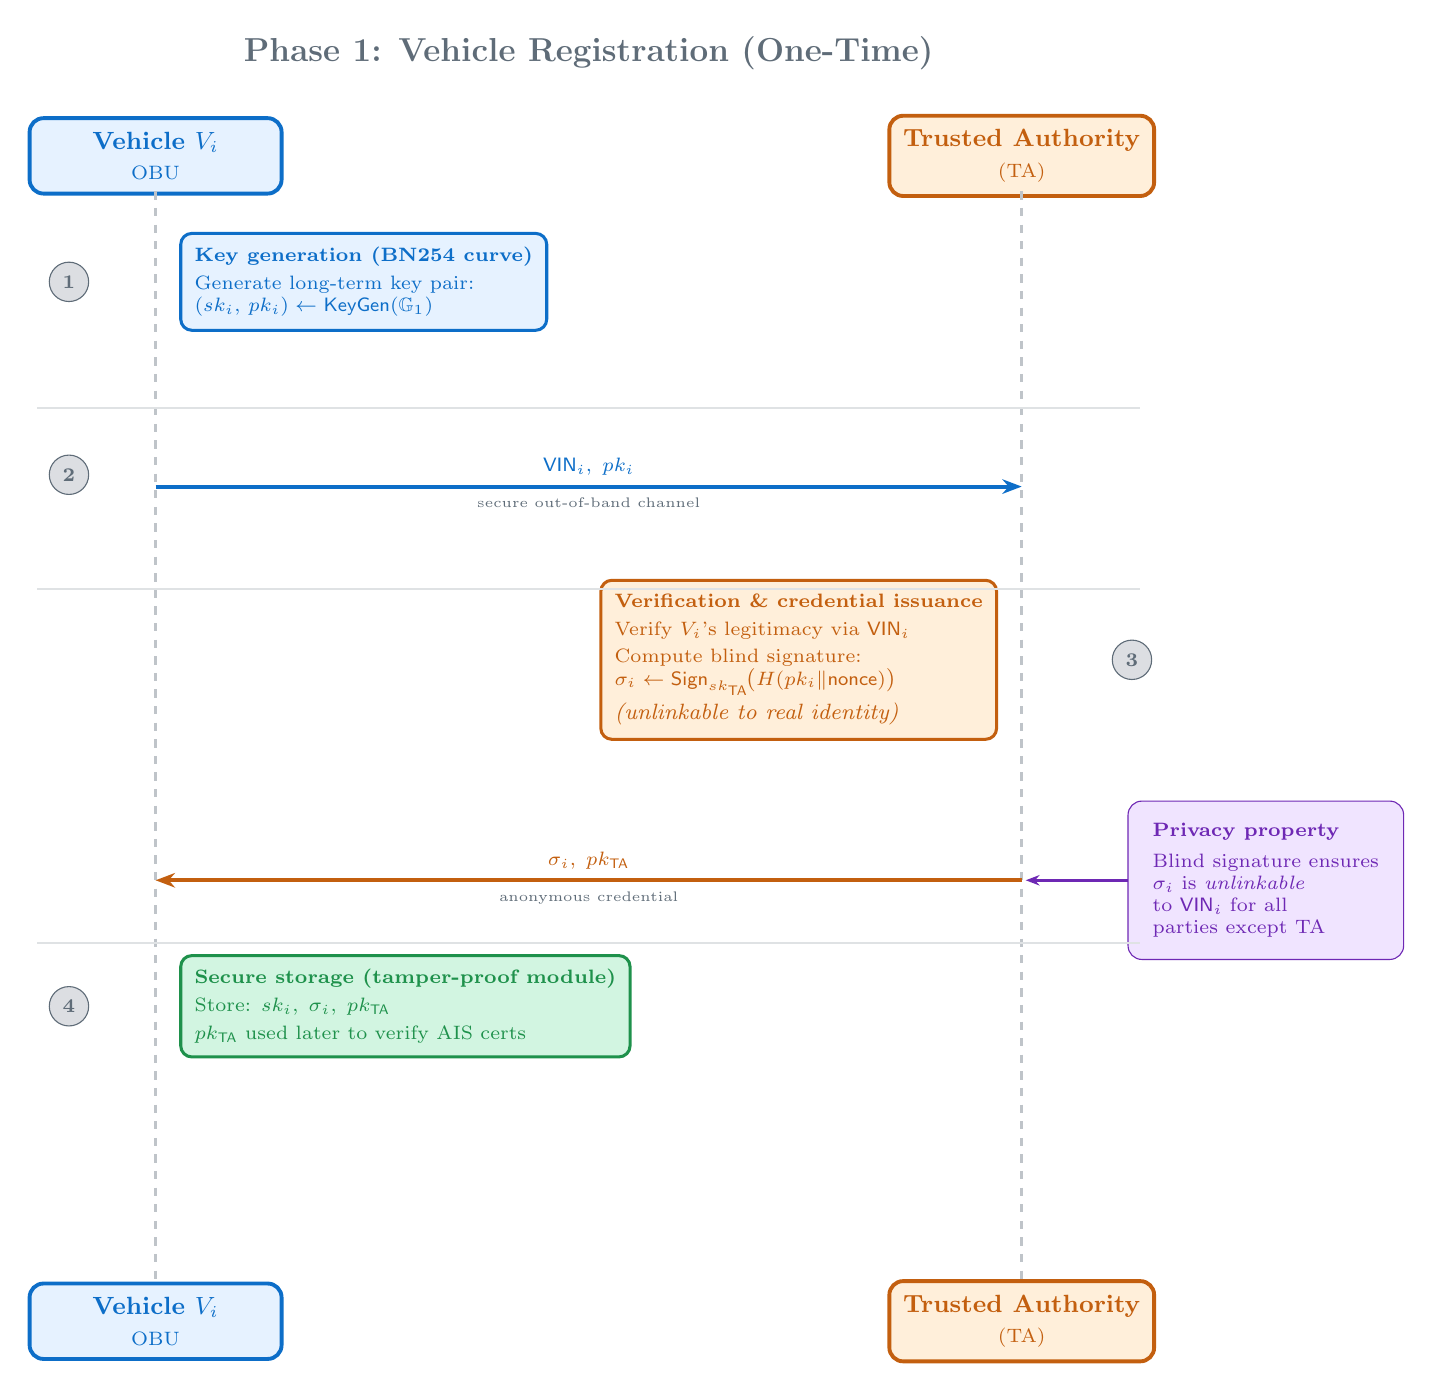
\begin{tikzpicture}

%% ============================================================
%%  ACTOR POSITIONS
%%  Vehicle Vi at x=0, TA at x=11
%% ============================================================
\def\Vx{0}
\def\Tx{11}

%% ----- Actor headers -----
\node[actorV] (Vi)  at (\Vx,  0) {Vehicle $V_i$\\{\scriptsize\normalfont OBU}};
\node[actorT] (TA)  at (\Tx,  0) {Trusted Authority\\{\scriptsize\normalfont (TA)}};

%% ----- Lifelines -----
\draw[lifeline] (\Vx, -0.45) -- (\Vx, -14.8);
\draw[lifeline] (\Tx, -0.45) -- (\Tx, -14.8);

%% ============================================================
%%  STEP 1 — Vi generates key pair  (y = -1.6)
%% ============================================================
\def\ya{-1.6}
\node[stepbubble] at (\Vx-1.1, \ya) {1};
\node[cboxV, anchor=west] (S1box) at (\Vx+0.3, \ya) {%
  \textbf{Key generation (BN254 curve)}\\[2pt]
  Generate long-term key pair:\\
  $(sk_i,\, pk_i) \leftarrow \mathsf{KeyGen}(\mathbb{G}_1)$
};

%% ============================================================
%%  STEP 2 — Vi sends identity + pk to TA  (y = -4.2)
%% ============================================================
\def\yb{-4.2}
\node[stepbubble] at (\Vx-1.1, \yb+0.15) {2};

%% message arrow Vi -> TA
\draw[msgarrowB] (\Vx, \yb) -- (\Tx, \yb)
  node[midway, above, font=\scriptsize\bfseries, text=cBlue]
    {$\mathsf{VIN}_i,\; pk_i$}
  node[midway, below, font=\tiny, text=cGray]
    {secure out-of-band channel};

%% ============================================================
%%  STEP 3 — TA verifies + issues blind credential  (y = -6.0)
%% ============================================================
\def\yc{-6.4}
\node[stepbubble] at (\Tx+1.4, \yc) {3};
\node[cboxT, anchor=east] (S3box) at (\Tx-0.3, \yc) {%
  \textbf{Verification \& credential issuance}\\[2pt]
  Verify $V_i$'s legitimacy via $\mathsf{VIN}_i$\\[2pt]
  Compute blind signature:\\
  $\sigma_i \leftarrow \mathsf{Sign}_{sk_{\mathsf{TA}}}\!\bigl(H(pk_i \| \mathsf{nonce})\bigr)$\\[2pt]
  {\footnotesize\textit{(unlinkable to real identity)}}
};

%% ============================================================
%%  STEP 3b — TA returns credential  (y = -9.2)
%% ============================================================
\def\yd{-9.2}
\draw[msgarrowO] (\Tx, \yd) -- (\Vx, \yd)
  node[midway, above, font=\scriptsize\bfseries, text=cOrange]
    {$\sigma_i,\; pk_{\mathsf{TA}}$}
  node[midway, below, font=\tiny, text=cGray]
    {anonymous credential};

%% ============================================================
%%  STEP 4 — Vi stores credentials  (y = -10.8)
%% ============================================================
\def\ye{-10.8}
\node[stepbubble] at (\Vx-1.1, \ye) {4};
\node[sbox, anchor=west] (S4box) at (\Vx+0.3, \ye) {%
  \textbf{Secure storage (tamper-proof module)}\\[2pt]
  Store: $sk_i,\;\sigma_i,\; pk_{\mathsf{TA}}$\\[2pt]
  $pk_{\mathsf{TA}}$ used later to verify AIS certs
};

%% ============================================================
%%  Property callout (right side)
%% ============================================================
\node[draw=cPurple, fill=cFillPurple, rounded corners=5pt,
      font=\scriptsize, align=left, inner sep=8pt,
      text=cPurple, minimum width=3.5cm]
  at (\Tx+3.1, -9.2) {%
    \textbf{Privacy property}\\[3pt]
    Blind signature ensures\\
    $\sigma_i$ is \textit{unlinkable}\\
    to $\mathsf{VIN}_i$ for all\\
    parties except TA
};

%% arrow from callout to credential arrow
\draw[-{Stealth[length=5pt]}, cPurple, line width=0.9pt]
  (\Tx+1.35, -9.2) -- (\Tx+0.05, \yd);

%% ============================================================
%%  TITLE
%% ============================================================
\node[font=\bfseries\large, text=cGray] at (5.5, 1.3)
  {Phase 1: Vehicle Registration (One-Time)};

%% ============================================================
%%  Horizontal separators (faint)
%% ============================================================
\foreach \yy in {-3.2, -5.5, -10.0} {
  \draw[cGray!20, line width=0.7pt] (-1.5, \yy) -- (12.5, \yy);
}

%% ============================================================
%%  Actor footers (bottom echo)
%% ============================================================
\node[actorV] at (\Vx,  -14.8) {Vehicle $V_i$\\{\scriptsize\normalfont OBU}};
\node[actorT] at (\Tx,  -14.8) {Trusted Authority\\{\scriptsize\normalfont (TA)}};

\end{tikzpicture}
\end{document}